\documentclass[12pt]{article}
\usepackage[utf8]{inputenc}
\usepackage{graphicx}
\usepackage{amssymb}
\usepackage{amsthm}
\usepackage{amsmath}
\usepackage{mathtools}
\renewcommand{\qedsymbol}{\rule{0.7em}{0.7em}}
\usepackage{tikz}
\usepackage[margin=0.8in]{geometry}
\setlength{\parskip}{1em}
\DeclarePairedDelimiter{\abs}{\lvert}{\rvert}
\DeclarePairedDelimiter{\floor}{\lfloor}{\rfloor}
\usepackage{tikz}
\usetikzlibrary{arrows.meta,positioning}

\usepackage[ruled]{algorithm2e}
\setlength{\algotitleheightrule}{0pt}

\renewcommand{\thesubsection}{\thesection.\alph{subsection}}

\title{CSC303 Assignment 1}
\author{Elias Volonakis, 1003936789}


\begin{document}

\maketitle

\section{}
\subsection{}
$A(G)$ is the adjacency matrix of $G$, $B(G) = A(G) + I$. Mathematically, this adds a diagonal of all 1s. With respect to the graph, the addition of $I$ means every vertex has a self-directed edge. In the final matrix $C = B(G)^2$, $c_{i,j}$ represents the number of possible paths from vertex $i$ to vertex $j$ of length 2, such that edges may be traversed more than once. The reason being that by definition, $s_{ij} = \sum^n_{k=\beta}{a_{i\beta}a_{\beta j}}$. Hence, a value of 1 is contributed to the sum only when both $a_{i\beta}$ and $a_{\beta j}$ are 1. That is, when the edges $(v_i, v_\beta)$ and $(v_\beta,v_j)$ are present edges in $G$. Those edges correspond to the 2 edges which are traversed in the path of length 2 between vertices $v_i$ and $v_j$.
\subsection{}
We may extend the result of 1a) to any $k \in \mathbb{N}$ to understand what is meant by $C^k$. That is, $c_{i,j} \in C^k$ represents the number of paths of length $k$ in the graph, such that edges may be traversed more than once. The reasoning for which is the same as 1a) extended to $k$. In 1a) $c_{i,j}$ was accumulated by determining if $(v_i, v_\beta)$ and $(v_\beta,v_j)$ are present edges in $G$. That would necessarily be a path of 2 edges $(v_i, v_\beta)$ and $(v_\beta,v_j)$. When taking the $k^{th}$ power of the adjacency matrix, $c_{i,j}$ is accumulated by determining if a path of $k$ edges $(v_i, v_\beta_1), ..., (v_\beta_k,v_j)$ are present in the graph. All possible paths of length $k$ between $v_i$ and $v_j$ will be counted in $c_{i,j} \in C^k$. 
\newline 
\newline 
If there is a row of nonzero entries of an adjacency matrix, then the graph must be connected because then there would exist a path from the vertex corresponding to that row to every other vertex in the graph. Hence, the entire graph would have to be connected. The minimum value of $k$ such that there will be a row of nonzero entries of an adjacency matrix is $\lceil \frac{d}{2} \rceil$. By the definition of the diameter of a graph, $d$ is the greatest distance between any pair of vertices. Such vertices will be connected by a path containing some intermediate vertex $\lceil \frac{d}{2} \rceil$ edges along the path. The distance from that vertex to any other vertex in the graph must be less that or equal to $\lceil \frac{d}{2} \rceil$, by the definition of diameter. Hence, the largest $k$ required is $\lceil \frac{d}{2} \rceil$. 

\newpage
\section{}
\subsection{}
The fewest number of days in which nodes $D$ and $G$ will become friends are 2. Observe, that $D$ and $G$ cannot become friends in 1 day, since they do not share a mutual friend. However, given triadic closure, it is possible to gain mutual friend in a day. There are multiple mutual friends, one being person $A$. After, a mutual friend is gained, there will be an open triangle containing $D$ and $G$. That means, the second day, closing that open triangle will be possible given triadic closure.  
\subsection{}
For $D$ and $K$ to be friends in 2 days, on day 1 they must gain a mutual friend. The only way this may occur is if there exists a friend 2 edges away from both $D$ and $K$. Such friends are only $F$ and $B$. Let $X$ denote the first method, that is connecting via friend $B$. Let $Y$ denote the second method, that is connecting via friend $F$. 
\newline 
\newline 
Method $X$ requires a friendship to form between $D$ and $B$ via $A$ and a friendship to form between $K$ and $B$ via $H$. Both of these events have a probability of $\frac{1}{2}$. Forming the final friendship of $D$ and $K$ via $B$, has a probability of $\frac{1}{2}$. Hence Method $X$ has a probability of $P(X) = \big ( \frac{1}{2} \big ) \cdot \big ( \frac{1}{2} \big ) \cdot \big ( 
 \frac{1}{2} \big ) = \frac{1}{8}$
\newline 
\newline 
Method $Y$ requires $D$ and $F$ to become friends on day 1. However, there are two ways for this to occur, namely the triangles $DCF$ or $DAF$. So to consider the probability of triangle $DFK$ forming, we must consider the probability of $DAF$ exclusive or $DCF$ forming. Exclusive or is required since once a friendship edge has been created, it cannot be again created via another mutual friend. The exclusive or is precisely: \\
(Probability of $DAF$ or $DCF$ forming) - (Probability of $DAF$ and $DCF$ forming)
\\
\\
So then the probability of the friendship $DF$ forming will be: $\big ( \big ( 1 - \big (
  \frac{1}{2} \big )^2 \big ) - \big ( \frac{1}{2} \big )^2
  \big ) = \frac{1}{2}$
\\ 
\\ 
Forming the frienship $KF$ via $G$ has a probability of $\frac{1}{2}$. Forming the final friendship of $D$ and $K$ via $F$, has a probability of $\frac{1}{2}$. Hence, Method $Y$ has a probability of $P(Y) = \frac{1}{8}$
\newline 
\newline 
We now ought to find the probability that of method $X$ exclusive or method $Y$ occurring, again because we can't have the same edge being created twice. We then must compute the probability as follows $P(X \cup Y) = P(X) + P(Y) - P(X \cap Y)$. Observe that $P(X \cap Y) = P(X) \cdot P(Y) = \frac{1}{8} \cdot \frac{1}{8} = \frac{1}{64}$. 
\newline 
\newline 
Necessarily then, $P(X \cup Y) = \frac{1}{8} + \frac{1}{8} - \frac{1}{64} = \frac{15}{64}$
\newline 
\newline 
So the probability of method $X$ exclusive or method $Y$ is $P(X \cup Y) - P(X \cap Y) = \frac{15}{64} - \frac{1}{64} = \frac{14}{64} = \frac{7}{32}$
\newline 
\newline 
Hence, the probability that $D$ and $K$ will be friends on the second day is $\frac{7}{32}$

 
\newpage
\section{}
\subsection{}
Below is a labeling of the edges of the graph, such that ($A,B$) is a strong edge and and the total number of strong edges are maximized. Edges are labeled S for strong and W for weak.  
\newline 
\newline 
\begin {tikzpicture}[-latex ,auto ,node distance =2 cm and 2 cm ,on grid ,
semithick ,
state/.style ={ circle ,top color =white , bottom color = processblue!20 ,
draw,processblue , text=black , minimum width =1 cm}]
\node[state] (B) {$B$};
\node[state] (G) [above left =of B]{$G$};
\node[state] (F) [below left =of B] {$F$};
\node[state] (A) [below right =of B] {$A$};
\node[state] (E) [below right =of F] {$E$};
\node[state] (D) [below right =of A] {$D$};
\node[state] (C) [above right =of A] {$C$};
\path (B) edge [-] node[above =0.15 cm] {W} (F);
\path (B) edge [-] node[above =0.15 cm] {S} (A);
\path (F) edge [-] node[below =0.15 cm] {S} (E);
\path (A) edge [-] node[below =0.15 cm] {W} (E);
\path (G) edge [-] node[above =0.15 cm] {W} (B);
\path (A) edge [-] node[above =0.15 cm] {W} (C);
\path (A) edge [-] node[below =0.15 cm] {W} (D);
\path (C) edge [-] node[right =0.15 cm] {S} (D);
\end{tikzpicture}
\subsection{}
By triadic closure, if there is an open triangle with 2 strong edges, the triangle must in fact be closed. Since ($A,B$) is strong, by strong triadic closure property, if ($G,B$) were also strong there would need to be an edge between ($G,A$), which there is not. The same argument holds for ($A,C$). That is, ($A,C$) cannot be strong since if it were there would need to be an between ($B,C$), which there is not. Again, the argument holds for ($A,D$). ($A,D$) cannot be strong since if it were, there would have to be an edge between ($B,D$), which there is not. ($B,F$) also cannot be strong since there is no edge between ($F,A$). Finally, ($E,A$) cannot be strong since there is no edge between ($F,A$). The remaining edges are $(F,E)$ and $(C,D)$. They do not form an open triangle with any strong edges, so they may be strong, as depicted in the graph above. That said, the maximum number of strong edges under these conditions are 3, as depicted above.
\newpage
\subsection{}
Below is a labeling of the edges of the graph, such that ($A,B$) is a strong edge and and the total number of strong edges are maximized. Edges are labeled S for strong and W for weak.  
\newline 
\newline 
\begin {tikzpicture}[-latex ,auto ,node distance =2 cm and 2 cm ,on grid ,
semithick ,
state/.style ={ circle ,top color =white , bottom color = processblue!20 ,
draw,processblue , text=black , minimum width =1 cm}]
\node[state] (B) {$B$};
\node[state] (G) [above left =of B]{$G$};
\node[state] (F) [below left =of B] {$F$};
\node[state] (A) [below right =of B] {$A$};
\node[state] (E) [below right =of F] {$E$};
\node[state] (D) [below right =of A] {$D$};
\node[state] (C) [above right =of A] {$C$};
\path (B) edge [-] node[above =0.15 cm] {W} (F);
\path (B) edge [-] node[above =0.15 cm] {W} (A);
\path (F) edge [-] node[below =0.15 cm] {S} (E);
\path (A) edge [-] node[below =0.15 cm] {W} (E);
\path (G) edge [-] node[above =0.15 cm] {S} (B);
\path (A) edge [-] node[above =0.15 cm] {S} (C);
\path (A) edge [-] node[below =0.15 cm] {S} (D);
\path (C) edge [-] node[right =0.15 cm] {S} (D);
\end{tikzpicture}
\newline 
\newline 
Again, by triadic closure, if there is an open triangle with 2 strong edges, the triangle must in fact be closed. Since, $(B,A)$ is weak, edges which form an open triangle with $(B,A)$ may be strong or weak. In particular, $(G,B)$ and $(A,C)$ can be strong without contradiction. Then, $(A,C)$, $(A,D)$, $(C,D)$ can all be strong, since those edges form a complete triangle. With this assignment, ($B,F$) and ($A,E$) may not be strong since there is no edge ($G,F$) and ($D,E$), respectively. What remains is edge $(F,E)$, which may be strong since it is not part of an open triangle with 2 strong edges. In the case that not all of $(A,C), (C,D)$ and $(A,D)$ were strong we would have stricly less strong edges in the graph. The reason being that if 2 edges are strong in the triangle $ACD$, then the third edge must likewise be strong. So if not all edges are strong, 2 must be weak. There are no other 2 edges that can be changed from strong to weak that would not cause a contradiction. That said, the maximum number of strong edges under these conditions are 5, as depicted above.  
\newpage
\section{}
\subsection{}
Consider the network depicted in figure 3.15, with the addition of the edge $(3,10)$. Recall that an edge is a bridge iff its removal disconnects the graph. Then, it is clear that the graph has no bridges, since the removal of any individual edges does not disconnect the graph. The edge $(3,10)$, however, is a local bridge. The reason being, when the edge is removed, the shortest path between vertices 3 and 10 has a length of 3. 
\subsection{}
Define the sets of vertices $A = \{1,2,3,4,5 \}$ and $B \{7,8,9,10,11\}$. Those sets partition the vertices of the graph into 2 disjoint regions that can only be connect via edges $(5,7)$ and $(3,7)$. 
\newline 
\newline
We wish to calculate the betweeness of edges $(5,7)$ and $(3,10)$. That is, we would like to determine the number of shortest paths between any two vertices which contains edge $(5,7)$ or $(3,10)$. By the symmetry of the graph, we may see that $(5,7)$ or $(3,10)$ must be contained in the shortest path from any vertex in $A$ to any vertex in $B$, and vica versa. As well, observe that vertex 3 is adjacent to all other vertices in $A$, and vertex 5 is adjacent to all vertices but vertex 1 in $A$. The same observation may be made for $B$, by the symmetry of the graph. That means, there will be more instances of $(3,10)$ appearing in a shortest path versus $(5,7)$ appearing in a shortest path. 
\newline 
\newline 
In particular, a shortest path beginning at 5 and ending at any vertex other than 11 will contain $(5,7)$. A shortest path beginning at 5 and ending at 11 may also contain $(5,7)$, however in that case the shortest path will not be unique. That is, a shortest path beginning at 5 and ending at 11 may contain $(3,10)$. The same is true for a shortest path beginning at 4 and ending at any vertex in $B$ other than 10 and 11. In the case the shortest path begins at 4 and ends at vertex 10 or 11, $(3,10)$ will be contained in the shortest path. A shortest path beginning at 3 will contain $(3,10)$. The shortest path between 3 and 7, however is not unique and could contain $(5,7)$ or $(3,10)$. A shortest path beginning at 2 and ending at 7, will contain $(5,7)$ by symmetry, because now 7 is an endpoint. A shortest path between 2 and 10, will contain $(3,10)$ by symmetry, because now 10 is an endpoint. Likewise, a shortest path between 2 and 11 will contain $(3,10)$ because 10 directly connects to 11, where as 5 does not. A shortest path between 1 and 7 contains $(5,7)$ or $(3,10)$, because 7 is an endpoint in the shortest path. However, one may observe that there are 3 shortest paths to consider, that is shortest paths $(1,3,5,7), (1,2,5,7,)$ and $(1,3,10,7)$. A shortest path beginning at 1 to any other vertex in $B$, since vertex 1 is adjacent to vertex 3. 
\newline 
\newline 
In the case there is not a unique shortest path, 0.5 will be added to the betweeness of both $(5,7)$ and $(3,10)$. Otherwise, 1 will be added to the betweeness of either $(5,7)$ or $(3,10)$, accordingly. Then we have the following values:
\newline 
\newline 
The betweeness of $(5,7)$ is 7(0.5) + 5 + $\frac{2}{3} = \frac{55}{6}$ \\ The betweeness of $(3,10)$ is 7(0.5) + 12 + $\frac{1}{3} = \frac{95}{6}$

\newpage 
\section{}
\subsection{}
The graph does provide evidence for homophily. That is, friendship and engagement in the same sport seems to be correlated since all volleyball players have at least 3 friends who also play volleyball and all hockey players have at least 2 friends who also play hockey. As well, all hockey players and volleyball players have at most 1 friend who plays the other sport. Specifically, only 3 hockey players and 3 volleyball players are friends. That is only $\frac{1}{2}$ of the hockey players and only $\frac{1}{2}$ of the volleyball players. 
\subsection{}
It is clear, that individuals who are friends who also play the same sport became friends due to homophily, that is their shared interest in the sport. The edges $(B,X)$, $(D,Y)$ and $(F,Z)$ represent different types of friendships. It is possible that those friendships formed due to other shared common interests. For instance, $(B,X)$ might represent individuals who also play music in a school band, $(D,Y)$ might represent individuals who participate in a school debating club and $(F,Z)$, might represent individuals who both enjoy computer programming. With no additional information about the Northern Ontario community, it is possible that those edges exist to a different homophily as explained. What might also be the case is that those edges exist due to immutable factors, such as if $(B,X)$, $(D,Y)$ and $(F,Z)$ are siblings who enjoy different sports. 
\subsection{}
If we add an edge between players $U$ and $V$, that edge could be explained by focal closure but not by triadic closure. The reason being is that they do not share any mutual friends, yet they both play hockey. Their friendship then will be created by their mutual interest in hockey, which is focal closure. 
\subsection{}
Observe that teenagers $B,D,F$ and $X,Y,Z$ are the only teenagers who have friends who play another sport. However, each teenager only has 1 friend who plays the other sport, since $(B,X)$, $(D,Y)$ and $(F,Z)$ are the pairs of friends. So all of these teenagers have a probability of $\frac{1}{4}$ of playing the other sport in one time step. That is, $B,D,F$ and $X,Y,Z$ are all equally likely to play the new sport in one time step.
\subsection{}
Warm-up routine $\tau$ will most likely be spread to the entire team. The reason being is that warm-up routine $\tau$ is a focus and it is possible then to have focal closure between the friends of $W$ and $U$, with the warm-up routine $\tau$. That is $X, Y, Z, V$ will probably all adopt warm-up routine $\tau$ due to focal closure because they are all friends with $W$. That means the entire hockey team will eventually adopt the warm-up $\tau$. That said, there is no volleyball player that has 2 hockey player friends. Thus warm-up $\tau$ will never spread to any of the volleyball players. 
\section{}
\subsection{}
\textbf{Focal Closure but Not Triadic Closure:}
\newline 
\newline 
\begin{tabular}{ |c|c|c| } 
\hline
Friendship & $i$-value & Probability \\
\hline
$B,D$ & 2 & $\frac{9}{25}$ \\
\hline
$C,F$ & 1 & $\frac{1}{5}$ \\ 
\hline
$A,B$ & 1 & $\frac{1}{5}$\\  
\hline
\end{tabular}
\newline 
\newline 
\newline 
\textbf{Focal Closure And Triadic Closure:}
\newline 
\newline 
\begin{tabular}{ |c|c|c|c|c| } 
\hline
Friendship & $f$-value & $i$-value & Probability \\
\hline
$A,F$ & 1 & 1 & $\frac{7}{15}$ \\ 
\hline
$B,C$ & 1 & 1 & $\frac{7}{15}$ \\ 
\hline
$B,G$ & 2 & 1 & $\frac{3}{5}$\\ 
\hline
$B,E$ & 1 & 1 & $\frac{7}{15}$ \\ 
\hline
$C,G$ & 1 & 1 & $\frac{7}{15}$ \\ 
\hline
\end{tabular}
\newline 
\newline 
\newline 
\textbf{Membership Closure:}
\newline 
\newline 
\begin{tabular}{ |c|c|c| } 
\hline
Friendship & $f$-value & Probability \\
\hline
$A, Club1$ & 2 & (1 - 0.7^2) = 0.51 \\
\hline
$B, Club2$ & 2 & (1 - 0.7^1) = 0.3 \\ 
\hline
\end{tabular}
\newpage
\subsection{}
Observe that the new student $C$ is immediately disqualified since he/she already attends club2. Then, what we would like to do is to see if $A$ or $C$ is most likely to start hanging out at one of the clubs. Observe then, since $A$ has 2 friends who frequent Club1, by \textbf{6.a}, the probability that there will be a membership closure between $A$ and Club1 is 0.51. Since $B$ has 1 friend who frequents Club2, by \textbf{6.a}, the probability that there will be a membership closure between $C$ and Club2 is 0.3. The probability $A$ or $B$ will go to the opposite clubs is zero, since neither of them have friends that go to opposite clubs, than those which were already mentioned. Since the probability of $A$ going to Club1 is greater than the probability of $B$ going to Club2, it is more likely that after first week $A$ will start going to one of the clubs. 
\newline 
\newline 
From this small group of students it seems that Club1 attracts dentistry students and Club2 seems to attract engineering students. With respect to homogeneous links, we may see that students who are connected to students studying similar disciplines. That is dentistry students are connected to other dentistry students and engineering students are connected to other engineering students. In the case the student study both disciplines, he/she is connected to another dentistry or engineering student, which also represents a homogeneous link. In fact, we may say there are 10 homogeneous links between students studying the same discipline. 
\subsection{}
It seems that $(D,E)$ is the most embedded edge. The reason being is that students $D$ and $E$ are both connected to student $A$. Likewise, both students $D$ and $E$ are dentistry students and frequent Club1. That gives us an embeddedness of 3, which is the highest of all edges in the social-affiliated network.  
\subsection{}
It seems that Club1 seems to attract students interested in dentistry and Club 2 seems to attract students interested in engineering. In particular, there are 2 dentistry students who frequent Club1 and there are 2 engineering students and 1 dentistry and engineering student who frequent Club2. 
\newpage
\section{}
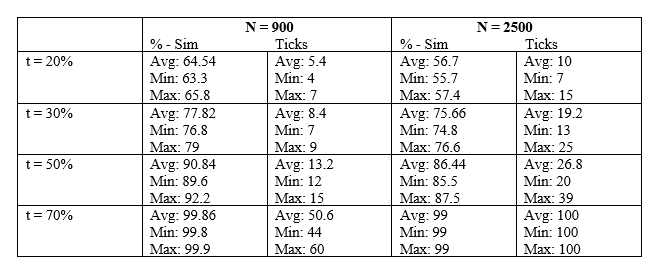
\includegraphics{CSC303Q7.PNG}
\newline
Examining the first column, $\textbf{N = 900}$, we may see that as threshold variable $t$ increases, so does the $\% - Sim$ and Ticks. That is, as $t$ increases from $20\%$ to $70\%$, the average $\%-Sim$ increases from 64.54 to 99.86 and the average Ticks increases from 5.4 to 50.6. The $\%-Sim$ increases since increased values $t$ will require a final higher $\%-Sim$. Likewise, the Ticks increased because the higher the value of $t$, the more time it will take to have a higher percent satisfied. Examining the second column, $\textbf{N = 2500}$, on average the $\%-Sim$ has decreased and the Ticks have increased, where $N$ has been increased from 900 to 2500. In general, when $N$ increases, the $\%-Sim$ is decreased on the same $t$ values. The reason being, with a greater population it will be harder to establish the same level of $\%-Sim$. That is it will need to be lower. The same phenomenon holds for $\%-Sim$ and Ticks. That is as $t$ increases from $20\%$ to $70\%$, so does the $\%-Sim$ and Ticks. It is also important to notice that the values $t = 70\%, N = 2500$ does not converge. For the purpose of the assignment, I have run the simulation for 100 ticks and each simulation reached a $\%-Sim$ of 99. The reason that the simulation of such high values of $t$ and $N$ do not converge is that the simulation is constantly trying to satisfy the value of $t$ for such a high population. In doing so, the simulation makes minute changes to the population, which increases and decreases the $\%-Sim$ by about 1$\%$. This fluctuates the value of $\%-Sim$ between 97 and 99. Finally after 100 Ticks, there are less minute changes and while the system does not completely stabilize, $\%-Sim = 99$ is reached.  







\end{document}
